\section{Accretion Disk Physics}

Consider a test particle orbiting in a Newtonian point mass potential. Its angular velocity $\Omega$ is given by
\begin{align}
    \Omega = \Omega_{\rm K} \equiv \sqrt{\frac{G M_*}{r^3}}, \label{eq:point_pot}
\end{align}
where $M_*$ is the central mass, $r$ is the orbital radius, $G$ is Newton's constant and $\Omega_{\rm K}$ signifies Keplerian rotation. 
Thus the orbital speed is a decreasing function of radius $v_\phi = r \Omega_{\rm K} \propto r^{-1/2}$.
Additionally, the specific angular momentum $h$ of the particle is given by
\begin{align}
    h = r \Omega^2 = \sqrt{G M_* r}, \label{eq:ang_mom}
\end{align}
and so we see that $h$ is an increasing function of radius as $h \propto r^{1/2}$.
Together the above quantities constitute a key feature of accretion disks; shearing stresses between annuli of material orbiting at slightly different radii, as well as other instabilities, allow for angular momentum transport within the disk. 
This means inner material may lose its angular momentum to the outer disk and accrete onto the star. 
Alternatively, the whole disk may lose angular momentum to its environment, for example through magnetised outflows that induce a torque on the disk.

\subsection{Fluid equations} \label{sec:fluid_eqns}

The structure and evolution of accretion disks are governed by the viscous and compressible continuity and momentum equations given by \citep[eg.][]{landau1987}
\begin{align}
    \partial_t \rho + \nabla \cdot (\rho \VF{v}) &= 0, \label{eq:fluid_cont} \\
    \partial_t \VF{v} + (\VF{v} \cdot \nabla) \VF{v} &= \frac{1}{\rho} \left( \nabla \cdot \VF{T} - \nabla P  \right) - \nabla \Phi_*, \label{eq:fluid_mom}
\end{align}
where $\rho, P$ and $\VF{v}$ are the fluid density, pressure and velocity respectively, $\VF{T}$ is the viscous stress tensor and $\Phi_*$ is the gravitational potential of the central point mass, which is assumed to dominate over the gravity of the disk. 
Following the review by \citet{papaloizou1995}, we find the corresponding equations of continuity and momentum that describe the evolution of a thin accretion disk.
Rewriting the continuity equation in cylindrical coordinates and expanding we find
\begin{align}
    \partial_t \rho + \nabla \cdot (\rho \VF{v}) &= \partial_t \rho + \frac{1}{r} \partial_r (r \rho v_r) + \frac{1}{r} \partial_\phi (\rho v_\phi) + \partial_z (\rho v_z) = 0.
\end{align}
Integrating this over all $\phi$ and $z$ gives
\begin{align}
    0 &= \int_0^{2\pi} \int_{-\infty}^\infty \left\{ \partial_t \rho + \frac{1}{r} \partial_r (r \rho v_r) + \frac{1}{r} \partial_\phi (\rho v_\phi) + \partial_z (\rho v_z) \right\} \dif{z} \dif{\phi} \\
    &= \partial_t \int_0^{2\pi} \int_{-\infty}^\infty \rho \dif{z} \dif{\phi} + \frac{1}{r} \partial_r \int_0^{2\pi} \int_{-\infty}^\infty r \rho v_r \dif{z} \dif{\phi}, \label{eq:int_cont}
\end{align}
where the third term vanishes and we neglect the fourth term assuming that $v_z \simeq 0$.
Carrying out the integration by assuming $v_r$ is independent of $\phi$ and $z$, equation \ref{eq:int_cont} becomes
\begin{align}
    \partial_t \Sigma + \frac{1}{r} \partial_r (r \Sigma v_r) = 0, \label{eq:1d_cont}
\end{align}
where we assume $\rho$ is independent of $\phi$, and the surface density $\Sigma$ is defined by 
\begin{align}
    \Sigma = \int_{-\infty}^\infty \rho \dif{z}.
\end{align} 
Equation \ref{eq:1d_cont} expresses that the total mass of the disk is conserved, even as material moves between adjacent annuli. 

Taking the $\phi$ component of the momentum equation gives
\begin{align}
    \partial_t v_\phi + (\VF{v} \cdot \nabla) v_\phi &= \frac{1}{\rho} \left( [\nabla \cdot \VF{T}]_\phi - \nabla_\phi P  \right) - \nabla_\phi \Phi_*.
\end{align}
From equation \ref{eq:point_pot} we see that $\nabla_\phi \Phi_* = 0$. If we assume that the disk is axisymmetric such that $v_\phi=r \Omega(r)$ then we find $\partial_t v_\phi = 0$ and $\nabla_\phi P=0$. 
The $\phi$ components of the remaining terms are given by \citep[eg.][]{armitage2022}
\begin{align}
    [(v \cdot \nabla) \VF{v}]_\phi &= v_r \frac{dv_\phi}{dr} + \frac{v_\phi v_r}{r}, \\
    [\nabla \cdot \VF{T}]_\phi &= \frac{1}{r^2} \partial_r (r^2 T_{r\phi}) + \partial_z T_{\phi z},
\end{align}
giving us
\begin{align}
    v_r \frac{dv_\phi}{dr} + \frac{v_\phi v_r}{r} &= \frac{1}{r^2 \rho} \, \partial_r (r^2 T_{r\phi}) + \frac{1}{\rho} \partial_z T_{\phi z}, \\
    \rho v_r \frac{dh}{dr} &= \frac{1}{r} \partial_r (r^2 T_{r\phi}) + r \partial_z T_{\phi z},
\end{align}
where in the second line we have used equation \ref{eq:ang_mom} and multiplied through by  $r \rho$. Integrating over all $\phi$ and $z$, and assuming that $T_{\phi z}$ vanishes as $z\rightarrow\pm\infty$, we obtain 
\begin{align}
    2\pi \frac{dh}{dr} r v_r \Sigma &= \partial_r \left( r^2 \int_0^{2\pi} \int_{-\infty}^\infty T_{r\phi} \dif{z} \dif{\phi} \right). \label{eq:z_van}
\end{align}
For a thin disk the $r\phi$ component of the viscous stress tensor is simply $\mu r \, d\Omega/dr$ where $\mu$ is the viscosity \citep[see review by][]{papaloizou1995}. 
Let us define the kinematic viscosity $\nu$ as 
\begin{align}
    \nu = \frac{1}{2 \pi \Sigma} \int_0^{2\pi} \int_{-\infty}^\infty \mu \dif{z} \dif{\phi}.
\end{align}
Thus equation \ref{eq:z_van} becomes
\begin{align}
    \Sigma v_r \frac{dh}{dr} &= \frac{1}{r} \partial_r \left( \Sigma r^3 \nu \frac{d\Omega}{dr} \right), \label{eq:1d_angmom}
\end{align}
which expresses that the total angular momentum of the fluid disk is conserved, under our various assumptions.

\subsection{Vertical density structure}

We may derive the vertical structure of the disk following the seminal review by \citet{pringle1981}. Taking the $z$ component of the momentum equation \ref{eq:fluid_mom}, again assuming $v_z \simeq 0$, giving
\begin{align}
    \frac{1}{\rho} \partial_z P = \partial_z \Phi_*,
\end{align}
ie. vertical hydrostatic equilibrium. 
Taking the pressure to be dominated by gas and assuming the disk is vertically isothermal with equation of state $P=c_s^2 \rho$ (which may not be a good approximation for protoplanetary disks, see \citet{pinte2018} and \citet{calahan2021}, for example) we find
\begin{align}
    \frac{c_s^2}{\rho} \partial_z \rho = - \frac{G M_* z}{\left(r^2 + z^2\right)^{3/2}} \simeq - \Omega_{\rm K}^2 z.
\end{align}
The approximate equality in the above applies assuming $z \ll r$. 
Solving this yields
\begin{align}
    \rho(r,z) &= \rho_0(r) \exp{\left( -\frac{z^2}{2 H^2} \right)}, \label{eq:vertical_rho}
\end{align}
where $\rho_0(r)$ is the density in the mid-plane at $z=0$, and we define the disk scale height $H = c_s/\Omega_{\rm K}$.
We may also find the relation between $\Sigma$ and $\rho$ by integrating equation \ref{eq:vertical_rho} over all $z$, yielding
\begin{align}
    \rho_0(r) = \frac{1}{\sqrt{2\pi} H} \Sigma(r).
\end{align}

\subsubsection{Rotation}

Taking the radial component of the momentum equation \ref{eq:fluid_mom}, neglecting viscosity, assuming $v_r \ll v_\phi$, and again taking the disk rotation to be axisymmetric
\begin{align}
    \frac{v_\phi^2}{r} &= \frac{G M_* r}{\left( r^2 + z^2  \right)^{3/2}} + \frac{1}{\rho} \partial_r P \simeq \frac{G M_*}{ r^2} + \frac{1}{\rho} \partial_r P, 
\end{align}
again in the second equality using $z \ll r$. Now, dividing each side by $r$ and using $c_s^2=dP/d\rho$
\begin{align}
    \Omega^2 &= \Omega_{\rm K}^2 + \left( \frac{c_s^2}{r^2} \right) \frac{r}{\rho} \frac{d \rho}{dr}, \\
    &= \Omega_{\rm K} \left[ 1 + \left(\frac{H}{r}\right)^2 \frac{d \ln{\rho}}{d \ln{r}}  \right]. \label{eq:rotation}
\end{align}
Thus we find Keplerian rotation to be a good approximation for disks if $H/r \ll 1$, in regions where $z \ll r$. Additionally, the correction term $d\ln{\rho}/d\ln{r}$ is negative in most astrophysical disks since the density usually decreases with radius, and so the true rotation is sub-Keplerian.

\subsection{Disk flaring}

An accretion disk is said to be flared if its aspect ratio $H/r$ increases with radius so that
\begin{align}
    \frac{H}{r} \propto r^\gamma, \quad \gamma > 0.
\end{align}
That is, the scale height of the disk increases with radius faster than just linearly so $H \propto r^{1+\gamma}$. 
A ``flat" disk has an aspect ratio independent of scale height, $\gamma=0$.
The physical condition for flaring is given by the effective temperature profile of the disk, which we can see by considering that for an ideal gas $c_s^2 \propto T_{\rm eff}$ \citep[eg.][]{pringle2007}, and so
\begin{align}
    \frac{H}{r} &= \frac{c_s}{r \Omega_{\rm K}} \propto \frac{T_{\rm eff}^{1/2}}{r^{-1/2}}.
\end{align}
Thus we see that whether a disk is flared depends on its temperature profile. 
It can be shown that all disks irradiated by a central object are flared \citep{kenyon1987}. 
Indeed, \citet{chiang1997} modelled passive disks around young stars and found approximately $T_{\rm eff} \appropto r^{-1/2}$, which yields $\gamma \simeq 1/4$. 
From equation \ref{eq:rotation}, we see that a consequence of aspect ratio increasing with radius is that the flow becomes increasingly sub-Keplerian in the outer disk.

\subsection{Viscous evolution}

%\begin{figure}
%    \centering
%    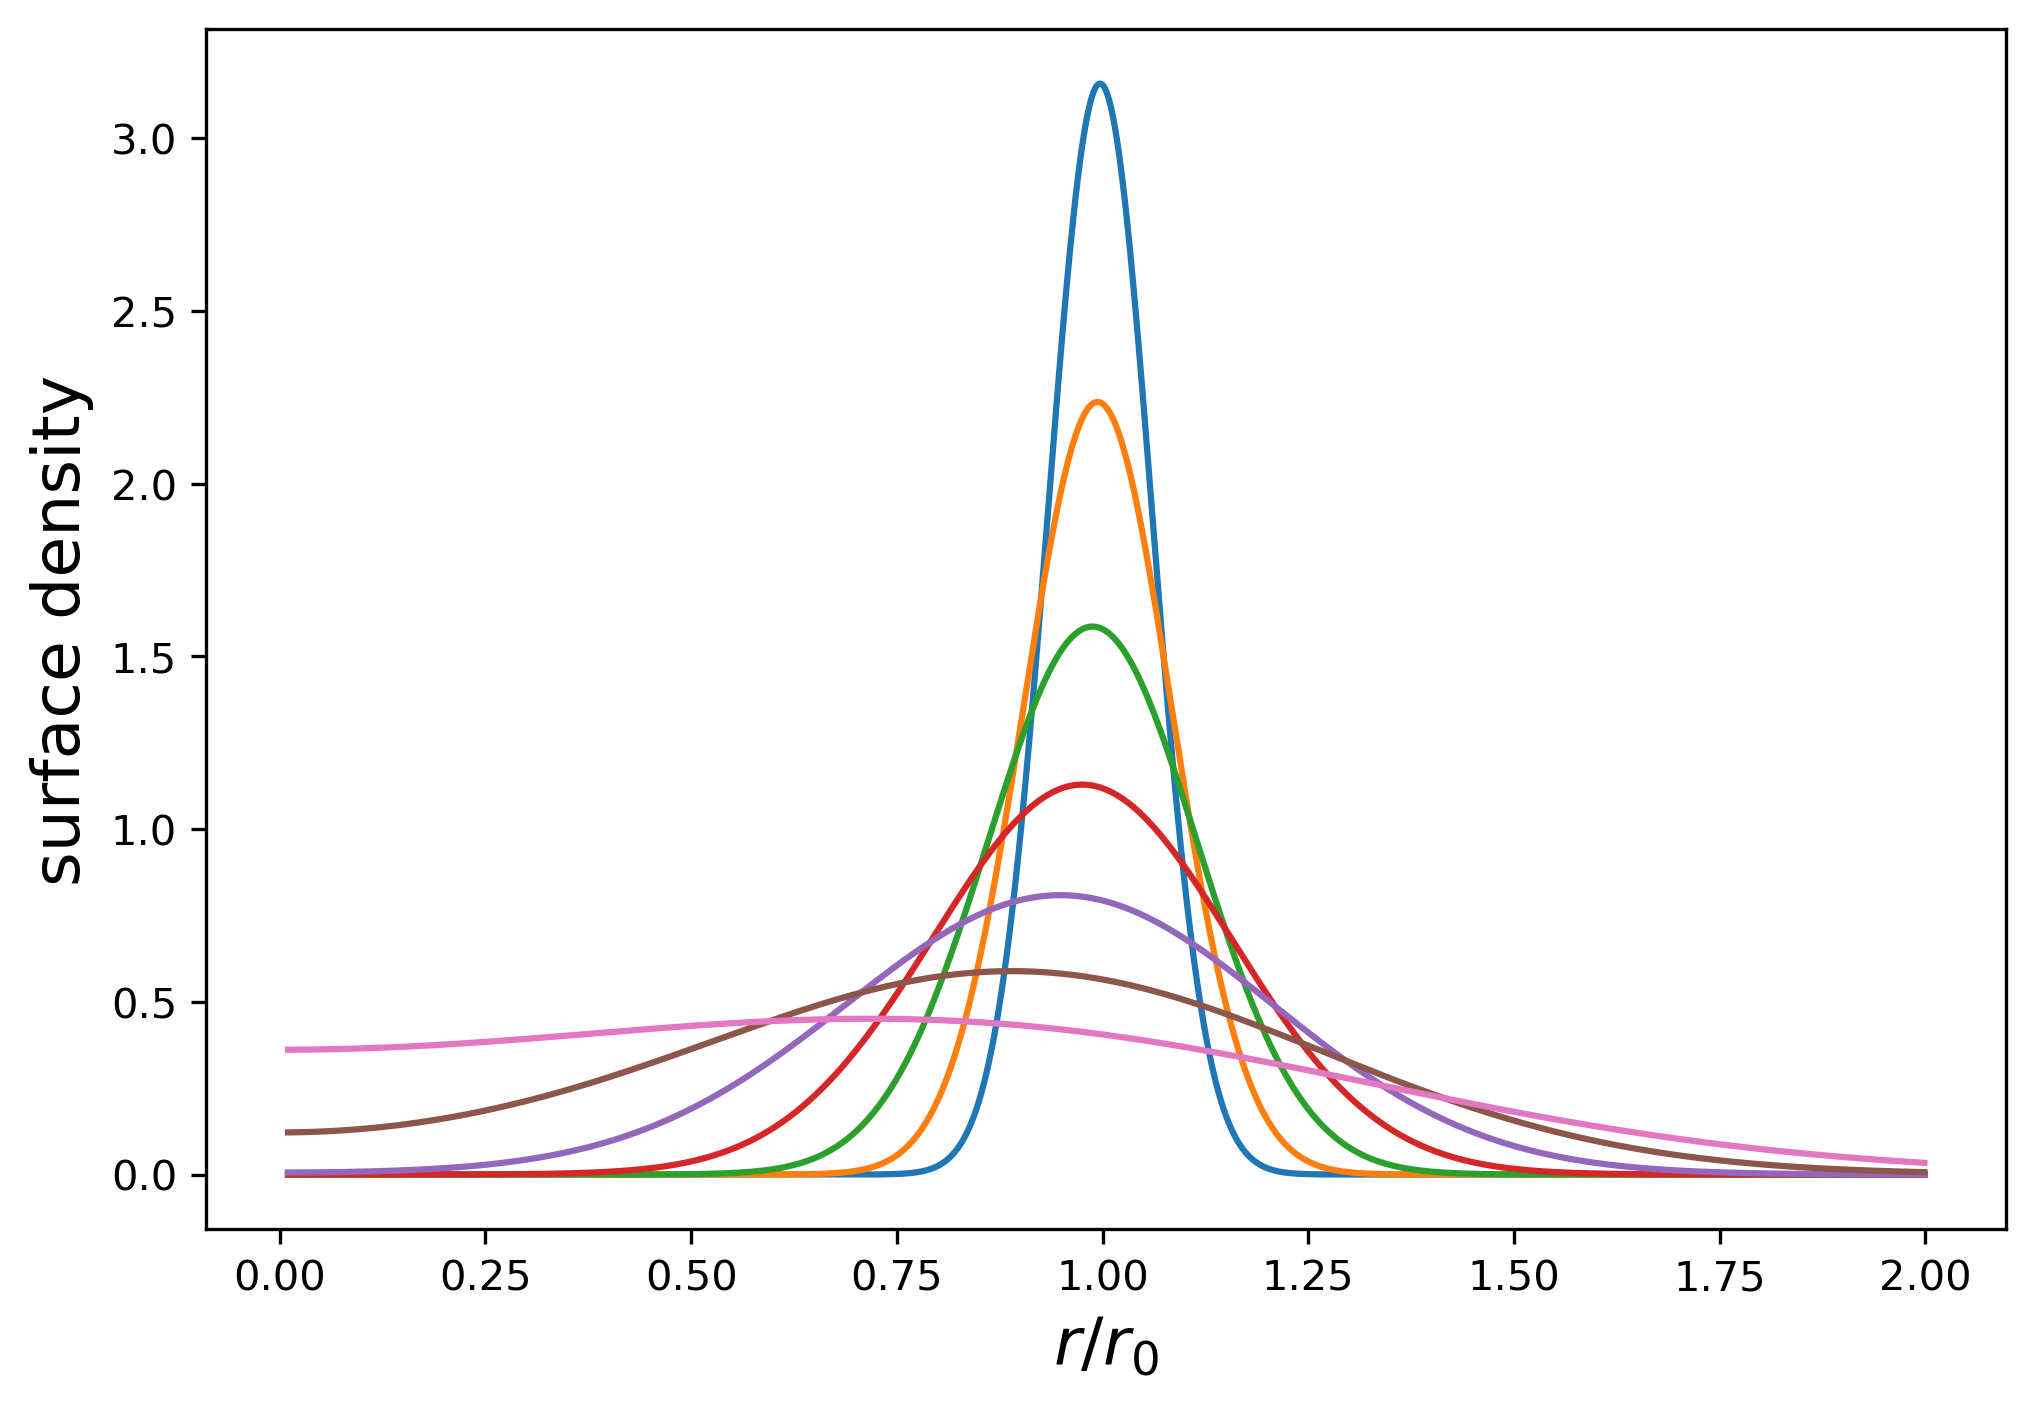
\includegraphics[width = 0.8\textwidth]{figures/armitage_ringspread.png}
%    \caption{The evolution of a ring of gas centred initially at $r=r_0$ according to equation \ref{eq:1d_evol}, as derived by \citet{lynden-bell1974}. Each curve is plotted from $\tau=0.008$ to $\tau=0.512$ with interval 0.084, where $\tau$ is dimensionless time \citep[figure from lecture notes by][]{armitage2022}. The diffusive nature of the evolution is clearly evident, with the overdense ring spreading out over time.}
%    \label{fig:ring_spreading}
%\end{figure}

Combining the mass and angular momentum conservation equations \ref{eq:1d_cont} and \ref{eq:1d_angmom}, and substituting the Keplerian forms for $\Omega$ and $h$ in equations \ref{eq:point_pot} and \ref{eq:ang_mom}, we find
\begin{align}
    \partial_t \Sigma &= \frac{3}{r} \partial_r \left[ \sqrt{r} \partial_r \left( \nu \sqrt{r} \Sigma  \right)  \right] \label{eq:1d_evol},
\end{align}
which is the surface density evolution equation for a thin, Keplerian disk. 
This is a partial differential equation, in the form of the 1D diffusion equation.
The diffusive property of the evolution equation is evident in the so-called ring spreading solution derived by \citet{lynden-bell1974} for the case where $\nu$ is constant, as shown in Figure %\ref{fig:ring_spreading}. 
We see that the solution involves the diffusion of a lot of mass to lower radii, while small amounts of mass carry the angular momentum away to very large radii.

In our analysis here and in section \ref{sec:fluid_eqns} we have implicitly used the effective viscous theory of accretion disks, where although angular momentum may physically be transferred by the magnerotational instability \citep{sano2000}, self-gravity \citep{kratter2016}, turbulent eddies \citep{klahr2003}, or other mechanisms, we assume that all of these can be captured considering the problem in terms of a fluid viscosity ($\nu$ in equation \ref{eq:1d_evol}).
Therefore, in order to model disk evolution, we must know how to determine the value of the viscosity $\nu$.
\citet{shakura1973} argued that it is physically consistent to parametrise the viscosity in terms of some constant $\alpha \lesssim 1$ as
\begin{align}
    \nu = \frac{2}{3} \alpha c_s H.
\end{align}
This is known as the $\alpha$-prescription. If $\nu \propto r^\beta$ for some constant $\beta$, then the surface density of a viscous accretion disk is given by \citep{lynden-bell1974}
\begin{align}
    \Sigma(r) = (2 - \beta) \frac{M_d}{2 \pi r_c^2} \left( \frac{r}{r_c} \right)^{-\beta} \exp{\left[ - \left(\frac{r}{r_c}\right)^{2-\beta} \right]},
\end{align}
which is an exponentially tapered power law. That is, the density drops approximately as a power law in $-\beta$ with radius for $r < r_c$, and for $r > r_c$ the exponential decay terms dominates. If we use the $\alpha$-prescription and the above definition for $\gamma$ then $\beta=2\gamma+\frac{3}{2}$. 
More commonly this is parametrised in terms of the effective temperature profile $T_{\rm eff} \propto r^{-q}$ for some constant $q$, giving $\beta = \frac{3}{2} - q$ \citep{hartmann1998}. 
If $q=1/2$ as in \citet{chiang1997}, then $\beta=1$.

\section{Spiral Density Waves}

\section{The Linear Disk Response}

\subsection{WKBJ Dispersion Relation}

Here we derive the dispersion relation for low-amplitude density waves propagating through a gas disk subject to a central gravitational potential, following the treatment from \citet{binney2008}.




\subsection{Lindblad Resonances}

\subsection{The Planet Wake}

\subsection{Additional Spiral Arms}

\section{Non-Linear Wake Evolution}

\subsection{The Burger's Equation}

\subsection{Angular Momentum Flux}

\section{Gap Formation}